\section{Introduction}
\label{introduction}

In the last decade GPUs computing has transformed the high performance 
computing, machine learning, and data analytics fields that were previously 
dominated by CPU-based 
installations~\cite{intersect360,cudnn,Lavin15b,SimonyanZ14a}. Many systems now 
rely on a combination of GPUs and CPUs to leverage high throughput data parallel 
GPUs with latency critical execution occurring on the CPUs. In part, 
GPU-accelerated computing has been successful in these domains because of native 
support for data parallel programming languages~\cite{CUDA7,OPENCL} that reduce 
programmer burden when trying to scale programs across ever growing data sets.

Nevertheless, with GPUs nearing the reticle limits for maximum die size and 
the transistor density growth rate slowing down~\cite{mooredead2016}, developers 
looking to scale the performance of their single GPU programs are in a 
precarious position. Multi-GPU programming models support explicit programming 
of two or more GPUs, but it is challenging to leverage mechanisms such as 
Peer-2-Peer access~\cite{NVIDIAP2P} or a combination of MPI and 
CUDA~\cite{NVIDIAMPI} to manage multiple GPUs. These programming extensions 
enable programmers to employ more than one GPU for high throughput computation, 
but they require re-writing of traditional single GPU applications,
slowing their adoption rate.

\begin{figure}[t]
	\centering
	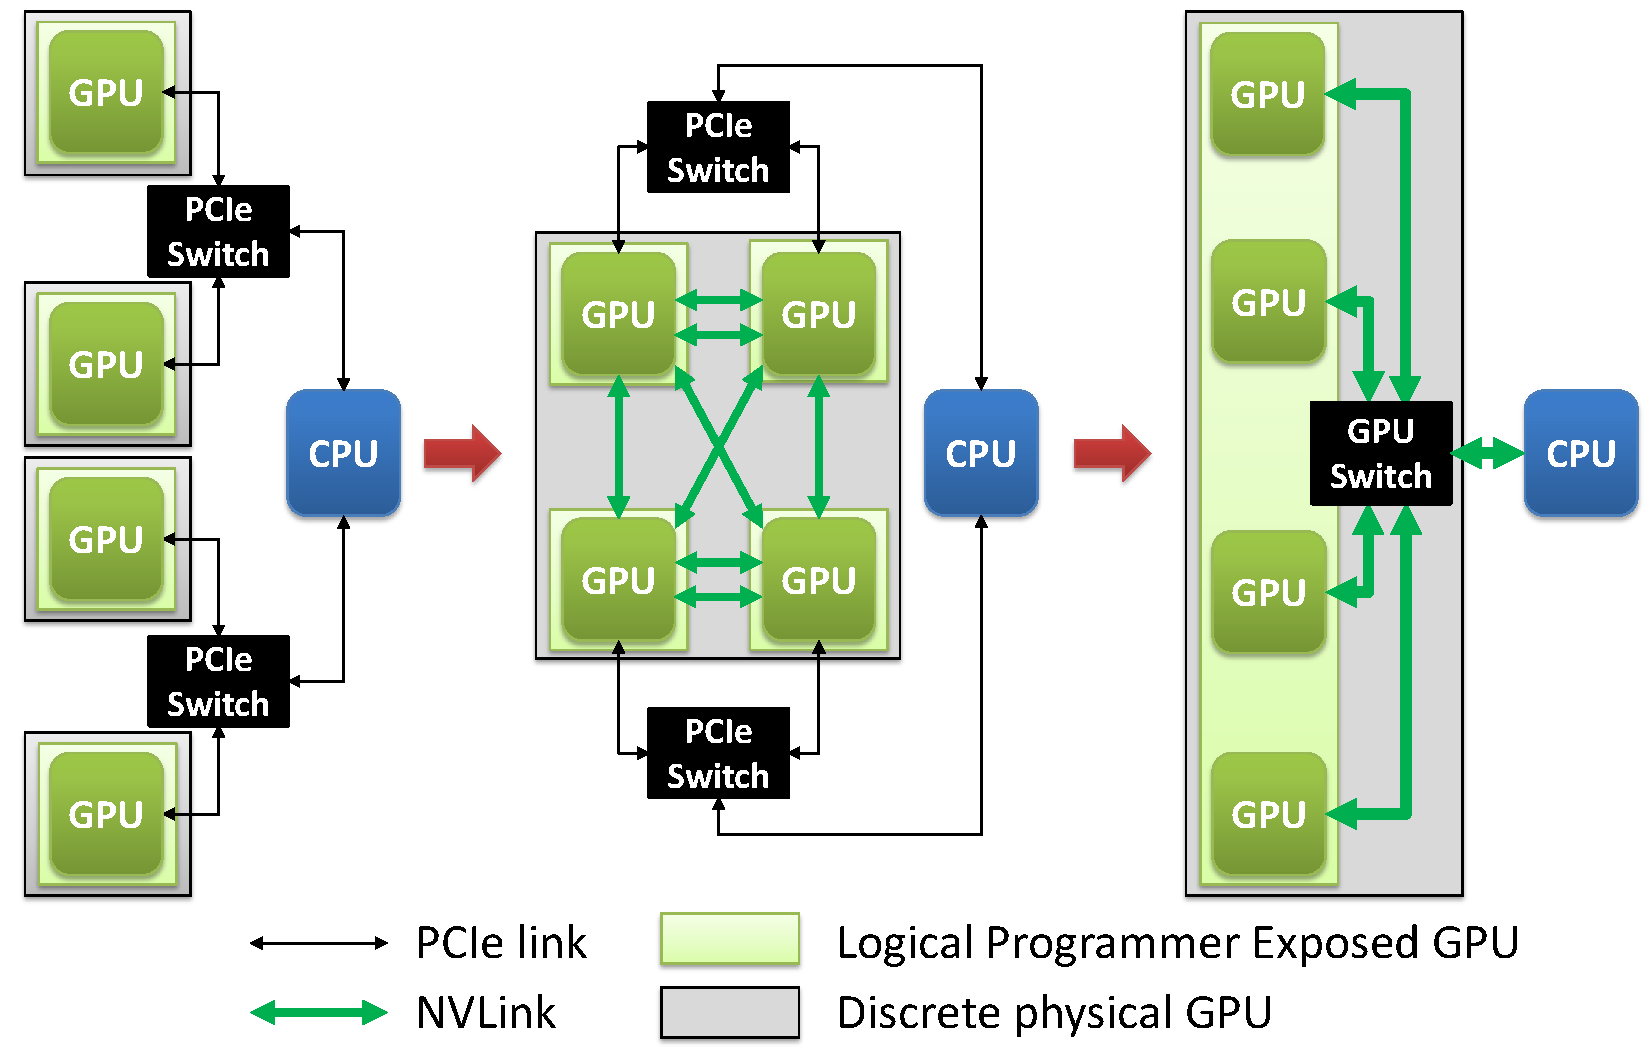
\includegraphics[width=1.0\columnwidth]{figures/inter_gpu_connections.pdf}
	\caption{The evolution of GPUs from traditional discrete PCIe devices to 
		single logical, multi-socketed accelerators utilizing a switched interconnect.}
	\label{fig:systemdiagram}
\end{figure}

High port-count PCIe switches are now readily available
and the PCI-SIG roadmap is projecting PCIe 5.0 bandwidth 
to reach \SI{128}{GB/s} in 2019~\cite{PCIeSwitches}. At the same time, GPUs are starting to expand 
beyond the traditional PCIe peripheral interface to enable more efficient interconnection
protocols between both GPUs and CPUs, such as AMD's Infinity Fabric or NVIDIA's Scalable Link Interface
and NVLink~\cite{dgx,SierraHPC,AMDINFINITYFABRIC,NVLINK,NVIDIASLI}.
Future high bandwidth GPU to GPU interconnects, possibly using
improved communication protocols, may lead to system designs with closely coupled
groups of GPUs that can efficiently share memory at fine granularity.

The onset of such multi-socket GPUs would provide a pivot point for GPU and system 
vendors. On one hand, vendors can continue to expose these GPUs as 
individual GPUs and force developers to use multiple
programming paradigms to 
leverage these multiple GPUs. On the other, vendors could expose multi-socket 
designs as a single non-uniform memory access (NUMA) GPU resource as shown in Figure~\ref{fig:systemdiagram}.  
By extending the single GPU programming model to multi-socket GPUs,  applications 
can scale beyond the bounds of Moore's law, while simultaneously retaining the 
programming interface to which GPU developers have become accustomed.

Several groups have previously examined aggregating multiple GPUs together under 
a single programming model \cite{lee2013transparent,Cabezas2015}; however this 
work was done in an era where GPUs had limited memory addressability and relied 
on high latency, low bandwidth CPU-based PCIe interconnects. As a result, prior work 
focused primarily on improving the multi-GPU programming experience rather than 
achieving highly scalable performance. Building upon this work, we propose a 
multi-socket \textit{NUMA-aware} GPU architecture and runtime that aggregates 
multiple GPUs into a single programmer transparent logical GPU. We show that in 
the the era of unified virtual addressing~\cite{UVM}, cache line addressable 
high bandwidth interconnects~\cite{NVLINK}, and dedicated GPU and CPU socket PCB 
designs~\cite{SierraHPC}, scalable multi-GPU performance may be achievable using 
existing single GPU programming models. This work, makes the following 
contributions:

\begin{itemize}
\item We show that traditional NUMA memory placement and 
scheduling policies are not sufficient for multi-socket GPUs to achieve 
performance scalability. We then demonstrate that inter-socket bandwidth will be 
the primary performance limiter in future NUMA GPUs.

\item By exploiting program phase behavior we show that inter-socket links (and 
thus bandwidth) should be dynamically and adaptively reconfigured at runtime to maximize link 
utilization. Moreover, we show that link policy must be determined on a per-GPU 
basis, as global policies fail to capture per-GPU phase behavior.

\item We show that both the GPU L1 and L2 caches should be made NUMA-aware 
and dynamically adapt their caching policy to minimize NUMA effects. We demonstrate
that in NUMA GPUs, extending existing GPU cache coherence protocols
across multiple sockets is a good design choice, despite the overheads.

\item We show that multi-socket NUMA-aware GPUs can allow traditional 
GPU programs to scale efficiently to as many as 8 GPU sockets, providing significant 
headroom before developers must re-architect applications to obtain additional performance.

\end{itemize}
